\titre{Objectif :} Etudier les algortithmes pour résoudre des problèmes géométriques. \\

\titre{Applications :}
\begin{enumerate}
	\item CAO
	\item Jeux vidéos en 2D et 3D
	\item Résistance des matériaux
	\item Robotique
	\item Réseaux
\end{enumerate}

\titre{Géométrie euclidienne :} Points et vecteurs du plan ou de l'espace. Cela suppose qu'on dispose d'un type nombre réel (problème : sensibilité aux perturbations). \\

\titre{Solutions à ces problèmes :}
\begin{enumerate}
	\item Méthodes algébriques
	\item Utiliser des opérations "pas dangereuses" (addition, soustraction), pour la multiplication il faut une précision doublée, la division est dangereuse
	\item Utiliser des nombres à précision arbitraire (fonctionne mais ralentit le code d'un facteur 100 à 200)
	\item Utiliser seulement le signe plutôt que la valeur
	\item Ne faire des calculs qu'en cas de "doute" (calcul paresseux)
	\item Tout faire avec des entiers (géométrie discrète)
\end{enumerate}
Il existe des bibliothèques standard pour faire ça (ex : CGal en C++)\\
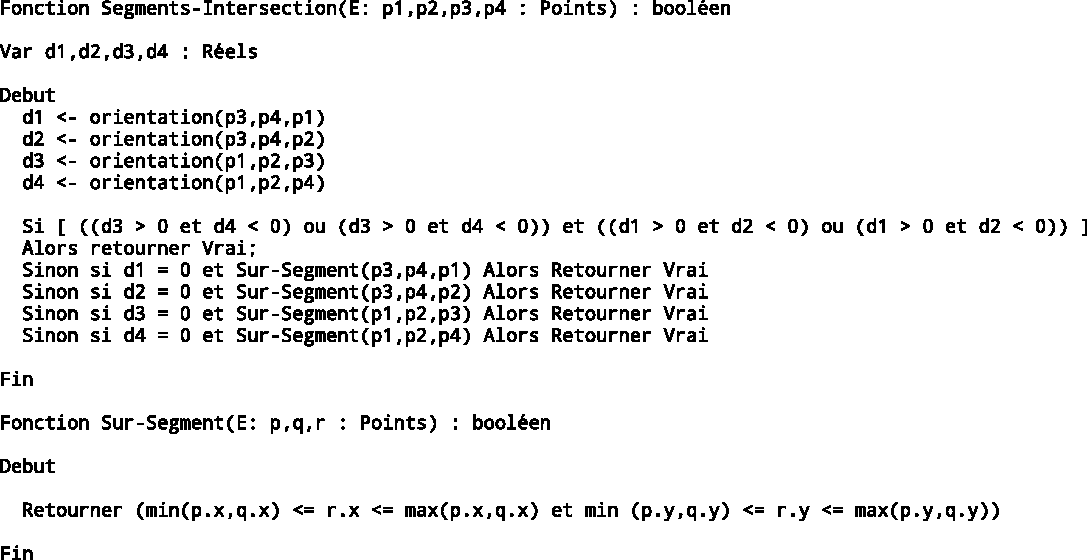
\includegraphics{Images/fig7.pdf}

\titre{Définition des éléments de base dans le plan :}
\begin{enumerate}
\item typedef struct { double x; double y; } Point; 
\item typedef struct { Point O; Point E; } Segment; C'est l'ensemble des points entre O et E $\rightarrow$ comment faire ça précisément ? On utilise les combinaisons linéaires sur O et E : $P = \alpha O + (1 - \alpha) E$ avec $\alpha \in [0;1]$ ie $[OE]=\{ \alpha O + (1 - \alpha) E \tq \alpha \in [0;1] \}$ cet ensemble est appelé ensemble des combinaisons convexes.
\item Longueur du segment $[OE]$ = distance euclidienne entre $O$ et $E$ = norme de $\vec{OE}$ = $\sqrt{(E.x - O.x)^2 - (E.y - O.y)^2}$. En géométrie algorithmique, on privilégie la distance au carrée (pour les erreurs et le temps de calcul).
\end{enumerate}

\titre{Question typique :} Etant donné un point $P$ et une droite $(P_1P_2)$, le point est il sur la droite, à sa gauche et à sa droite ? On utilise le déterminant de $\vec{P_1P_2},\vec{P_1P}$ (positif : $P$ est à gauche, négatif : $P$ est à droite, nul : $P$ est sur la droite.) Cela s'appelle la fonction d'orientation : retourne $(P_2.x - P_1.x)(P_2.y - P_1.y) - (P_2.y - P_1.y)(P.x - P_1.x)$\\

\titre{Question :} Comment déterminer si deux segments consécutifs $[P_1P_2]$ et $[P_2P_3]$ forment un vira	ge à droite ? Réponse on regarde si Orientation($P_1,P_2,P_3$) est négatif. \\

\titre{Question :} Comment déterminer si deux segments sont sécants ? $[P_1P_2]$ et $[P_3P_4]$ s'intersectent si $P_1$ et $P_2$ ne sont pas du même côté de $[P_3P_4]$ et que $P_3$ et $P_4$ ne sont pas du même côté de $[P_1P_2]$\\

\titre{Polygone :} Courbe du plan refermée sur elle même, composée d'une suite de segments de droite consécutifs appelés les côtés du polygone. Un sommet est l'intersection de 2 côtés consécutifs, et le nombre de sommets est égal au nombre de côtés.\\

\titre{Polygone simple :} Seuls les segments consécutifs s'intersectent en leurs extrémités.\\

\titre{Structure de données :} On caractérise un polygone par la séquence de ses sommets (modulo un choix de sommet de départ arbitraire)\\

\titre{Propriété :} Si un polygone est simple, alors il découpe le plan en deux zones connexes : l'intérieur et l'extérieure.\\

\titre{Exercice :} Ecrire un algorithme de complexité en $O(n^2)$ qui décide si un polygone donné sous forme de tableau est simple. ($n=$ nombre de côtés).\\
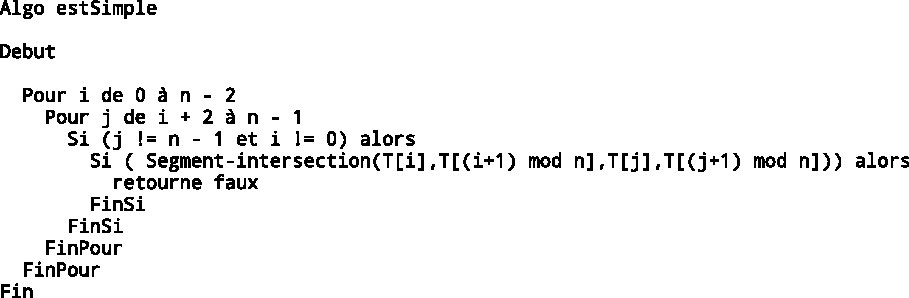
\includegraphics{Images/fig8.pdf}\\

\titre{Question :} Complexité minimale pour déterminer la liste des points d'intersections d'un polygone ($\Omega (n^2)$) (cf polygone type grille). \\

\titre{Complexité minimale pour décider si un polygone est simple :} $\theta(n\ln n)$ (algo pour tester si il y a une intersection au sein d'un ensemble quelconque de segments adapté au cas des polygones). \\

\titre{Algorithme par balayage d'une droite :} On se donne une direction de calcul (l'axe des abscisses), et on fait "avancer un droite virtuelle" (perpendiculaire à l'axe des ordonnées) \\

\includegraphics[width=150px]{Images/fig9.pdf} \\
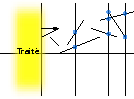
\includegraphics[width=150px]{Images/fig10.pdf} \\

\includegraphics{Images/fig11.pdf} \\

\titre{Question :} Etant donné un point x, est-ce que x est à l'intérieur d'un polygone simple ? Astuce depuis x on trace un rayon vers l'infini et on compte les intersections avec le bord (si je pars de l'intérieur c'est impair, sinon c'est pair) \\
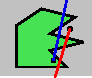
\includegraphics[width=150px]{Images/fig12.pdf} \\

\titre{Convexité :} Une partie $C$ du plan est convexe si et seulement si $\forall x,y \in C$ le segment $[xy]$ est inclus dans $C$. (exemple : algo GJK pour la détection de collisions)\\

\titre{Utilisation :} A partir d'une forme non convexe, on cherchera son enveloppe convexe. \\

\titre{Remarque :} Si $P$ est un ensemble de points ou un polygone, alors le contour de $\mathrm{Conv}(P)$ est un polygone simple. \\

\titre{Propriété :} Dans un polygone simple convexe, deux côtés consécutifs font toujours un "virage à gauche". \\

\titre{Propriété :} Si $P_iP_{i+1}$ est un côté de l'enveloppe convexe des points $(P_i)_{i\in\{0,\ldots,n-1\}}$, alors tous les autres points dont du côté gauche.\\

\titre{Algo naïf de calcul de l'enveloppe convexe :}
